\subsection{Feature extraction} \label{subsec:feature-extraction}

The feature extraction module receives a multi-channel audio signal of a fixed
length and outputs a \emph{feature frame}. Which is defined as the group of
vectors of features extracted from a finite number of samples. One vector per
\emph{extractor} used. \Cref{fig:datasets-frames} illustrates how an audio
signal is divided into frames. The number of samples per frame can be tied
together with the sample rate of the audio signal to define frames in terms of
time. Frame duration is one of the parameters of the dataset as well as the
number of features extracted per frame. \Cref{table:datasets-parameters} lists
all the different parameters that define a dataset.

\begin{figure}
    \centering
    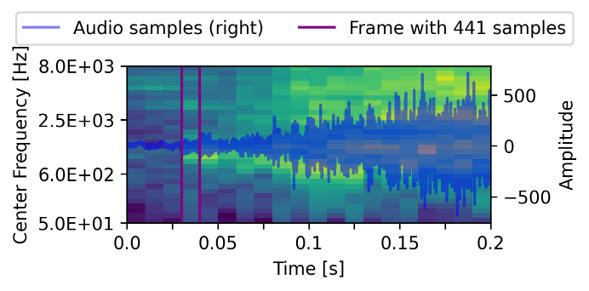
\includegraphics[width=\linewidth]{\subdir/frames.png}
    \caption[Audio frames]{Audio signal (in {\color{blue} blue}) over its
        features extracted from frames with a duration of 10 ms with a single
        \nameref{subsubsec:gammatone-filterbank} extractor.}
    \label{fig:datasets-frames}
\end{figure}

The term \emph{extractor} will be used to abstract the system used to extract
features from audio data. Although in this work only one type of extractor has
been implemented and tested. Additional feature extractors, like the
traditional Mel-frequency Cepstrum Coefficients (MFCC) or a simple Short-Time
Fourier Transform, can be easily implemented as the
\nameref{subsec:feature-extraction} module is decoupled from the
\nameref{sec:prediction-model}. 

This work opts to use a feature extractor based on
\nameref{subsubsec:gammatone-filterbank} since the performance of
classification systems relying on MFCCs is greatly reduced in the presence of
noise \cite{marchegiani2018a}.

\subsubsection*{Gammatone filterbanks} \label{subsubsec:gammatone-filterbank}

An approximation to the human cochlear frequency selectivity originally
introduced in \cite{GTF1998}. Time-independent features are obtained by
filtering the audio waveform with a bank of gammatone band-pass filters. The
impulse response of a gammatone filter centered at frequency $f_c$ is given by
\cref{eq:gammatone-filter-impulse}, where $n$ indicates the order of the filter
which largely determines the slope of the filter's skirts; and $b$ is the
bandwidth of the filter and largely determines the duration of the impulse
response; $a$ is the amplitude and $\phi$ is the phase.

\begin{equation}
    g(t, f_c) = a t^{n-1}e^{-2 \pi b t} \cos{2 \pi f_c t + \phi}
    \label{eq:gammatone-filter-impulse}
\end{equation}

This work implements a bank of fourth order gammatone filters with its
corresponding bandwidth $b$ of 1.019 ERB where ERB is the equivalent
rectangular bandwidth scale \cite{GLASBERG1990103}. It is based on a Matlab MEX
function implemented in C by \citeauthor{CorrelogramMa2007}
\cite{CorrelogramMa2007}, which at the same time is based on
\citeauthor{Cooke1993ModellingAP}'s Ph.D work \cite{Cooke1993ModellingAP}. The
filters are distributed over a predefined frequency range linearly on the ERB
scale. The number of filters used is equivalent to the number of features to be
extracted. 